\documentclass{article}

\usepackage[a4paper, left=1.5cm, right=1.5cm, top=2cm, bottom=2cm]{geometry}

\usepackage{../../../../components/components}
\usepackage{hyperref}
\usepackage{fancyhdr}


% Configuration des en-têtes et pieds de page
\pagestyle{fancy}
\fancyhf{} % reset tout

\fancyhead[L]{DL2 Math-Info ASF4}
\fancyhead[C]{Algèbre}
\fancyhead[R]{2025-2026}

\fancyfoot[L]{Ewen Rodrigues de Oliveira}
\fancyfoot[R]{\thepage}

\begin{document}

\docTitle{Chapitre 8 : Isométries et orientation des espaces euclidiens en dimensions 2 et 3}

\section{Orientation d'un espace vectoriel}

On définit une relation d'équivalence sur les bases \textit{ordonnées} d'un espace vectoriel $E$.
On dira : $\mathcal{B} = (e_1, \ldots, e_n) \sim (e_1', \ldots, e_n') = \mathcal{B}'$ si et seulement si $det P_{\mathcal{B} \to \mathcal{B}'} > 0$.

\training{Démontrer qu'il s'agit d'une relation d'équivalence.}
\noindent \carreaux{10}

\definition{
    Une orientation d'un espace vectoriel $E$ est un choix de l'une des classes d'équivalence pour cette relation.
}

\example{
    $E = \mathbb{R}^2$ muni de $(\overleftarrow{i}, \overleftarrow{j})$ la base canonique.\\ L'orientation "classique" de $\mathbb{R}^2$ est la classe d'équivalence de $(\overleftarrow{i}, \overleftarrow{j})$ pour $\sim$.
    
    \begin{center}
        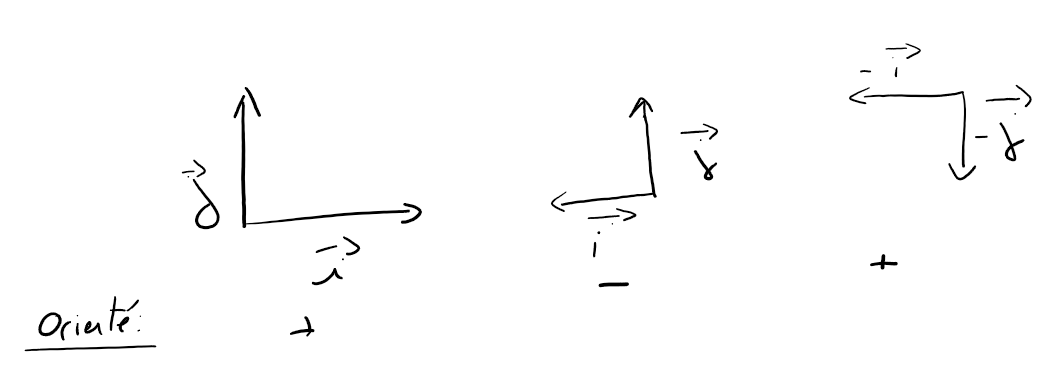
\includegraphics[width=0.5\textwidth]{./images/eg1.png}
        \captionof{figure}{Schéma de différentes orientations de $\mathbb{R}^2$}
    \end{center}
}

\example{
    $E = \mathbb{R}^3$ muni de $(\overleftarrow{i}, \overleftarrow{j}, \overleftarrow{k})$ la base canonique.\\ L'orientation "classique" de $\mathbb{R}^3$ correspond à la "règle de la main droite".
    \begin{center}
        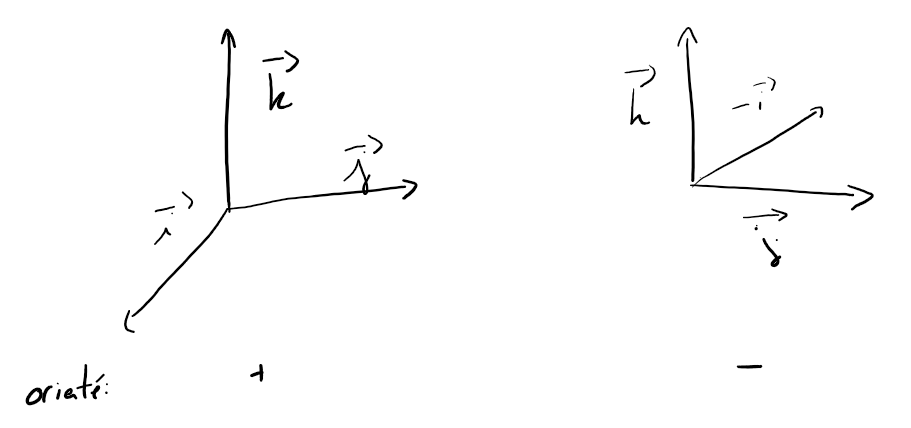
\includegraphics[width=0.5\textwidth]{./images/eg2.png}
        \captionof{figure}{Schéma de différentes orientations de $\mathbb{R}^3$}
    \end{center}
}

\section{Espaces euclidiens et produits mixtes}

\definition{
    Un espace euclidien orienté est un espace euclidien muni d'une orientation.
}

\newpage
\tableofcontents

\end{document}